\documentclass[12pt,letterpaper,english,bibliography=totocnumbered, abstract=on]{scrartcl}

\usepackage{indentfirst}
\usepackage[titletoc]{appendix}
\usepackage[T1]{fontenc}
\usepackage[latin9]{inputenc}
\usepackage{color}
\usepackage{babel}
\usepackage{verbatim}
\usepackage[unicode=true,pdfusetitle,
bookmarks=true,bookmarksnumbered=false,bookmarksopen=false,
breaklinks=true,pdfborder={0 0 0},pdfborderstyle={},backref=false,colorlinks=true]
{hyperref}
\hypersetup{linkcolor=blue,citecolor=blue,urlcolor=blue}

\usepackage{booktabs}
\usepackage{multirow}
\usepackage{adjustbox}
\usepackage{threeparttable}
\usepackage[table]{xcolor}
\usepackage{csquotes}
\usepackage{soul} % for hiliting text: \hl

\usepackage[backend=biber, style=authoryear, maxbibnames=99, dashed=false]{biblatex}
\setlength\bibitemsep{2\itemsep}
\addbibresource{CRB.bib}

\usepackage{pdfpages}
\usepackage{float} % Allows use of H to place floats

\usepackage{pgfgantt}

\usepackage{framed}

\usepackage{datetime2}

\usepackage{courier}
\usepackage{listings}
\lstset{basicstyle=\tiny\ttfamily,
	columns=fullflexible,
	%basewidth=0.51em,
	frame=single}

% Prevent page breaks within paragraphs
% https://tex.stackexchange.com/questions/21983/how-to-avoid-page-breaks-inside-paragraphs
\widowpenalties 1 10000

\begin{document}

\titlehead{TECHNICAL REPORT}

\title{Set Up for Automated Roadside Video Surveys for Detecting and Monitoring Coconut Rhinoceros Beetle Damage on Rota}

\author{Aubrey Moore}

\maketitle

%\footnote{The most recent version of this document can be downloaded from\\
%	\url{https://github.com/aubreymoore/roadside/blob/master/docs/roadside/roadside.pdf}.}

\newpage

\section{Project Overview}

A novel method for detecting and monitoring coconut rhinoceros beetle (CRB) damage to coconut palms has been developed and is being used on Guam. This method uses a smart phone mounted on a vehicle to record roadside videos which are georeferenced using the phone's GPS receiver.  Digital image analysis of these videos detects coconut palms, assigns a damage index to each palm and locates v-shaped cuts indicative of CRB damage.

This CRB damage detection and monitoring system will be tested on Rota following the recent range expansion of the CRB infestation on the island. The goal for this is early detection of CRB damage symptoms to trees visible from roadways so that control measures can be deployed. 

A kit consisting of a smart phone and accessories configured for the survey has been shipped to Rota by air freight. The plan is to mount the smart phone sent from Guam on a vehicle and record videos by driving all major roads in both directions. Videos will be recorded using the OpenCamera app which has been programmed to saved on a large microSD card installed in the phone. Another app, GPSLogger will automatically record the geographical position of the phone. It is expected that the islandwide survey can be completed within 2 or 3 days.

Upon return of the equipment to Guam, data will be analysed and results will be made available on an interactive, online map. 

\section{Equipment List}

\begin{itemize}
	\item Samsung Galaxy S7 smart phone equipped with: a 256 GB microSD card, OpenCamera app, GPSLogger app, and Clinometer app installed. 
	\item Magnetic ball and socket mount
	\item Charging cable
	\item Cigarette lighter socket adapter
\end{itemize}

\section{Mounting the Smart Phone on a Vehicle}

Preliminary work showed that mounting the smart phone externally produces much better results than mounting the phone internally as a dash cam. This eliminates problems cause by dirty windshields and internal reflections. The smart phone is mounted externally using a ball and socket anchored using a strong magnet. Optimal placement of the smart phone camera appears to be above the right-hand corner of the windshield (passenger side in the US). 

\section{Setting the Direction of View Angles for the Smart Phone Camera}

The smart phone camera needs to be set up to point 45 degrees to the right of the direction of travel of the vehicle and 15 degrees above horizontal. 

For instruction on setting these angles, please refer to the short YouTube video at\\ \url{https://www.youtube.com/watch?v=Pa-UslJV6BI}.

\section{Recording Roadside Videos}

\begin{itemize}
	\item Drive to the start of the survey.
	\item Mount the phone on the over the passenger side windscreen with angles set as above.
	\item Connect the phone to the vehicle's power supply using the charging cable and cigarette lighter adapter. 
	\item Ensure that the GPSlogger is recording positional data. GPSlogger is programmed to start whenever the phone is started. There may be a lag of a few minutes before a good satellite fix is made.
	\item Start the OpenCamera app and start a video recording. OpenCamera has been programmed so that the bright "flashlight" LED flashes to give a visual signal whenever a video is being recorded.
	\item IMPORTANT: Ensure that the camera is not "zoomed in". Zooming in OpenCamera is controlled by a slider which may be adjusted accidentally (See Fig. \ref{fig:zommedinout}). 
	\item Drive the planned survey route in one direction and then drive the same route in the opposite direction so that both sides of the road are covered.
	\item Completely turn off the phone at the end of the day.  
\end{itemize}

For more info or to report problems, please contact:

Aubrey Moore

Email: aubreymoore@guam.net

Cell phone: 671-686-5664

\begin{figure}
	\centering
	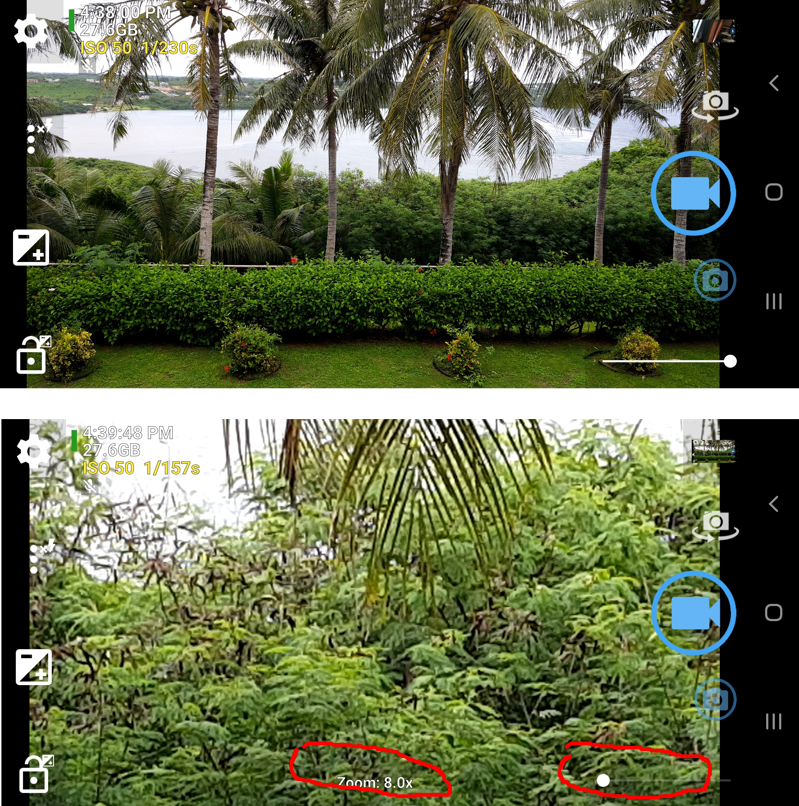
\includegraphics[width=0.7\linewidth]{../images/zommed_in_out}
	\caption{OpenCamera should appear as in the top screen capture. The bottom image
		shows OpenCamera set incorrectly, with the lens zoomed in.}
	\label{fig:zommedinout}
\end{figure}


 






\end{document}
